\documentclass{article}

\usepackage{algorithm}
\usepackage{algorithmic}
\usepackage{graphicx}
\usepackage{marvosym}
\usepackage{dingbat}

\title{The Conjugate Gradient Method}
\date{}

\begin{document}
\maketitle

\section{The Conjugate Gradient}

The Conjugate Gradient (CG) is an iterative method for the solution
for sparse, symmetric and positive-definite linear systems. Remember,
sparse matrices are matrices where most of the coefficients are equal
to zero. The zero coefficients are not explicitly stored in memory and
are not considered in all the operations involving the matrix; this
allows to reduce the memory consumption as well as the complexity of
matrix operations.

The CG method receives in input a starting solution $x=x_0$ and
refines it until the desired accuracy is reached (for example, until
the norm of the residual is smaller than a certain threshold $\|r\|_2
= \|b-Ax\|_2 < \varepsilon$ and/or when the number of iterations
exceeds a maximum value). In its basic form, the CG is described by
the algorithm below:

\begin{algorithmic}[1]
  \REQUIRE a matrix $A$, a right-hand side $b$ and a starting solution $x_0$
  \STATE $d_0 = r_0 = b-Ax_0$
  \WHILE {$\|r_i\|_2 > \varepsilon$ and $i < itmax$}
  \STATE $\alpha_i = \frac{r^T_i r_i}{d^T_iAd_i}$
  \STATE $x_{i+1} = x_i + \alpha_id_i$
  \STATE $r_{i+1} = r_i - \alpha_iAd_i$
  \STATE $\beta_{i+1} = \frac{r^T_{i+1} r_{i+1}}{r^T_i r_i}$
  \STATE $d_{i+1} = r_{i+1} + \beta_{i+1}d_i$
  \ENDWHILE
\end{algorithmic}

The method only requires four basic operations:
\begin{enumerate}
\item matrix-vector product $y = \alpha Ax + \beta y$
\item dot-product $v = x^Ty$
\item vector 2-norm $v = \|x\|_2$
\item vector sum $y = \alpha x + \beta y$
\end{enumerate}
where $y$ and $x$ are dense vectors, $A$ is a sparse matrix, $\alpha$,
$\beta$ and $v$ are scalars.

The objective of this exercise is to parallelize each of these four
operations independently using OpenMP in order to accelerate the
Conjugate Gradient. The mathematical details of the CG method are, in
this context, not important and can be neglected.

\section{Sparse Matrix Format}

Because the zero coefficients of the matrix must not be stored, a
standard 2D array cannot be used for storing a sparse matrix. 
In this exercise, sparse matrices are represented in Compressed Sparse
Row (CSR) format that consists of three arrays:

\begin{itemize}
\item \texttt{val}: this array of size \texttt{nz} contains the
  nonzero coefficients of the matrix sorted by rows (all the
  coefficients in the first row, then all those in the second row
  etc.)
\item \texttt{colind}: this array of size \texttt{nz} contains the
  column indices for the coefficients in the \texttt{val} array
\item \texttt{rowptr}: this array of size \texttt{n+1} contains
  pointer to the beginning of each row inside the \texttt{val} and
  \texttt{colind} arrays. For example \texttt{rowptr[3]=4} means that
  the first coefficient of row 3 is the 4th element of array
  \texttt{val} and its column index is equal to
  \texttt{colind[4]}. Therefore, all the coefficients of row
  \texttt{i} are between positions \texttt{rowptr[i]} and
  \texttt{rowptr[i+1]-1}.
\end{itemize}
where \texttt{n} is the size of the matrix and \texttt{nz} is the number
of nonzero coefficients in the matrix.

Here is an example:

\vspace{0.5cm}

\begin{minipage}{0.4\linewidth}
\begin{displaymath}
   A=\left[\begin{array}{ccccc}
   1 & 0 & 3 & 0 & 0\\
   4 & 2 & 0 & 1 & 0\\
   0 & 0 & 7 & 0 & 2\\
   8 & 2 & 5 & 0 & 0\\
   0 & 3 & 0 & 4 & 0\\
  \end{array}\right]
\end{displaymath}
\end{minipage}%
\begin{minipage}{0.6\linewidth}
  \centering
  \includegraphics[width=\textwidth]{csr}
\end{minipage}

\newpage

The sparse matrix-vector product $y = \alpha Ax + \beta y$ is computed
with the following routine: % in Figure~\ref{fig:spmv}.
% \begin{figure}[!h]
  % \centering
\small
\begin{verbatim}
void spmv(int n, int *rowptr, int *colind, double *val, 
          double alpha, double *x, double beta, double *y){

  int i, j;

  for(i=0; i<n; i++){
    /* for each row... */
    y[i] = beta*y[i];
    for(j=rowptr[i]; j<rowptr[i+1]; j++){
      /* for each coefficient in the row... */
      y[i] += alpha*val[j]*x[colind[j]];
    }
  }
  return;
}
\end{verbatim}
% \caption{\label{fig:spmv} The sparse matrix-vector product.}
% \end{figure}
\normalsize

Note that each iteration of the outer loop handles one row of the
matrix and each iteration of the inner loop handles one coefficient of
a row.


\section{Package content}
In the \texttt{ConjugateGradient} directory you will find the
following files:
\begin{itemize}
\item \texttt{conjugategradient.c}: this file contains the main
  program that reads a matrix $A$ from a file, generates a right-hand
  side $b$ and computes the solution $x$ of the system $Ax=b$ using
  the Conjugate Gradient method. {\bf This file should not be
    modified}.
\item \texttt{kernels.c}: this file contains the subroutines that
  perform the four basic operations described above. {\bf This is the
    only file that must be modified} as described below.
\item the remaining files contain auxiliary routines and can be safely
  ignored.
\end{itemize}

The code can be compiled with the \texttt{make} command: just type
\texttt{make} inside the \texttt{ConjugateGradient} directory; this
will generate a \texttt{main} program that can be run like this:

\begin{verbatim}
$ ./main matrix_file
\end{verbatim}

where \texttt{matrix\_file} can be \texttt{matrix1.rb},
\texttt{matrix2.rb} or \texttt{matrix3.rb}. When executed, the main
program will read the matrix $A$ from the file, generate the
right-hand side $b$ and find the solution $x$ of the linear system
$Ax=b$ using the CG method. It will print the norm of the residual
$\|r\|_2 = \|b-Ax_i\|_2$ every 10 iterations and, at the end, will
print the total number of iterations done, the residual of the final
solution and the CG execution time.

% The matrices can be found in the
% \texttt{/mnt/n7fs/ens/tp\_abuttari/TP\_SysCo/Matrices\_BE/}
% directory. Before running the program for the first time, just make a
% copy of these files into the \texttt{ConjugateGradient} directory:

% \begin{verbatim}
% $ cp /mnt/n7fs/ens/tp_abuttari/TP_SysCo/Matrices_BE/matrix*.rb .
% \end{verbatim}

\section{Assignment}
\begin{itemize}
\item {\huge \Keyboard} Use OpenMP to parallelize the four subroutines in the
\texttt{kernels.c} file. In case you used the \texttt{omp parallel
  for} construct, consider using different scheduling types.
\item \smallpencil Analyze and compare the performance of the parallel
  code using one or two threads. Report in the \texttt{responses.txt}
  file the number of iterations and the execution time for the three
  example matrices \texttt{matrix1.rb}, \texttt{matrix2.rb} and
  \texttt{matrix3.rb}. Comment on the observed results: did you
  observe any speedup (reduction of the execution time) using 2 or 4
  threads instead of 1? did you observe any difference in the number
  of iterations using 2 or 4 threads instead of 1?  Is the method
  still converging when using 2 or 4 threads? Did you observe any
  difference when using a dynamic scheduling instead of a static one?
  can you explain this difference?
\end{itemize}


\paragraph{Advice.}
\begin{itemize}
\item Note that some operations are easier to parallelize than
  others. The vector sum routine \texttt{axpby} is the easiest, the
  \texttt{dot} and \texttt{norm2} are a bit more difficult and,
  finally, the matrix-vector product \texttt{spmv} is the hardest. It
  is recommended to begin with the easier routines first and to
  validate the correctness of the result each time one routine is
  parallelized.
\item It is reasonable to expect that the number of iterations to
  convergence is slightly different when using 2 (or more) threads
  instead of 1. The difference, however, should be very small (not
  more than 10 iterations for the given test matrices). Therefore, if
  you observe a big difference in the number of iterations or if the
  method does not converge anymore it means that the code was not
  correctly parallelized.
\end{itemize}



















\end{document}




%%% Local Variables: 
%%% mode: latex
%%% TeX-master: t
%%% End: 
